\Article{11}
Let us now turn more closely to our subject itself. If, for the modulus $m=a+bi$, the numbers $f,f',f''$, etc., are such that, first, they are all incongruent to one another modulo $m$, and, second, every integer must necessarily be congruent to one of them, we call the
\SourceLeaf{326}
collection of numbers $f,f',f''$, etc., the system of primitive residues of $m$. Their number is always $=aa+bb$.

\Article{12}
The system of primitive residues can be formed in many ways. The simplest is to choose the points inside the square $0,m,(1+i)m,im$, but the following must also be included:
\begin{enumerate}
\item[I.] the point or quantity $0$;
\item[II.] all points on two boundary lines that are not opposite one another.
\end{enumerate}
Instead of taking all points on one of the $4$ boundary lines, one can also take them on several at once.

This choice of points on the boundary lines, if any lie on them, can be made in several ways that satisfy the above conditions. The following method is the simplest.

On the boundary line $0,m$, take all points between $0$ and $\frac12m$, inclusive, and on the boundary line $0,im$ all points from $\frac12im$ to $im$, exclusive; proceed similarly on the other two.

\Needspace{10\baselineskip}
These two methods can be represented visually as follows:
\begin{center}\resizebox{.85\textwidth}{!}{\begin{tikzpicture}[x=1bp,y=-1bp,line cap=round,line join=round]
\path[use as bounding box] (0,0) rectangle (1230,440);
\begin{pgfinterruptboundingbox}
\draw[line width=2.2bp] (228,69) -- (72,214) -- (218,366) -- (373,219) -- (326,168);
\draw[line width=2.2bp] (322,163) -- (257,96);
\draw[line width=2.2bp] (250,90) -- (228,69);
\draw[line width=2bp] (148,136) circle[radius=5bp];
\draw[line width=2bp] (304,140) circle[radius=5bp];
\draw[line width=2bp] (297,284) circle[radius=5bp];
\draw[line width=2bp] (152,290) circle[radius=5bp];
\node[inner sep=0pt,outer sep=0pt,anchor=center] at (53,214) {\scalebox{3.5}{\ensuremath{m}}};
\node[inner sep=0pt,outer sep=0pt,anchor=center] at (228,48) {\scalebox{3.5}{\ensuremath{(1+i)m}}};
\node[inner sep=0pt,outer sep=0pt,anchor=center] at (399,220) {\scalebox{3.5}{\ensuremath{im}}};
\node[inner sep=0pt,outer sep=0pt,anchor=center] at (213,387) {\scalebox{3.5}{\ensuremath{0}}};
\draw[line width=2.2bp] (839,229) -- (993,77) -- (1143,234) -- (987,378) -- cycle;
\draw[line width=2bp] (878,197) circle[radius=5bp];
\draw[line width=2bp] (906,155) circle[radius=5bp];
\draw[line width=2bp] (951,112) circle[radius=5bp];
\draw[line width=2bp] (1023,116) circle[radius=5bp];
\draw[line width=2bp] (1069,151) circle[radius=5bp];
\draw[line width=2bp] (1112,193) circle[radius=5bp];
\draw[line width=2bp] (869,270) circle[radius=5bp];
\draw[line width=2bp] (915,303) circle[radius=5bp];
\draw[line width=2bp] (956,344) circle[radius=5bp];
\draw[line width=2bp] (984,373) circle[radius=5bp];
\draw[line width=2bp] (1024,352) circle[radius=5bp];
\draw[line width=2bp] (1055,309) circle[radius=5bp];
\draw[line width=2bp] (1098,269) circle[radius=5bp];
\node[inner sep=0pt,outer sep=0pt,anchor=center] at (819,229) {\scalebox{3.5}{\ensuremath{m}}};
\node[inner sep=0pt,outer sep=0pt,anchor=center] at (991,54) {\scalebox{3.5}{\ensuremath{(1+i)m}}};
\node[inner sep=0pt,outer sep=0pt,anchor=center] at (1166,236) {\scalebox{3.5}{\ensuremath{im}}};
\node[inner sep=0pt,outer sep=0pt,anchor=center] at (978,397) {\scalebox{3.5}{\ensuremath{0}}};
\end{pgfinterruptboundingbox}
\end{tikzpicture}
}\end{center}

\Article{13}
If the following are excluded from the primitive points:
\begin{enumerate}
\item[I.] only the point $0$, when $a$ is even and $b$ odd, or the reverse;
\item[II.] the points $0$ and $\frac12(1+i)m$, when $a$ and $b$ are both odd;
\item[III.] the four points $0,\frac12m,\frac12(1+i)m,\frac12im$, when $a$ and $b$ are both even,
\end{enumerate}
we call the remaining points proper primitive points and the excluded ones improper. The number of the former is therefore
\[
\begin{array}{rrcl}
\text{in case}&\mathrm{I}&=&aa+bb-1\\
&\mathrm{II}&=&aa+bb-2\\
&\mathrm{III}&=&aa+bb-4
\end{array}
\]
and is thus always divisible by $4$.

\SourceLeaf{327}
\Article{14}
These proper primitive points can be divided into $4$ classes $F,F',F'',F'''$ so that
\[
\begin{array}{llll}
iF\equiv F'&iF'\equiv F''&iF''\equiv F'''&iF'''\equiv F\\
-F\equiv F''&-F'\equiv F'''&-F''\equiv F&-F'''\equiv F'\\
-iF\equiv F'''&-iF'\equiv F&-iF''\equiv F'&-iF'''\equiv F''
\end{array}
\]
The following extremely important theorem now holds.

Let $M$ be a number with no factor in common with $m$. Of the numbers $MF$, the number belonging to the class $F$ is $n$,
\[
\begin{array}{cc}F'&n'\\F''&n''\\F'''&n'''\end{array}
\]
and let the least residue of $n'+2n''+3n''$ modulo $4$ be $=N$, so that $N$ equals one of the $4$ numbers $0,1,2,3$. Under this assumption, $N$ is \emph{independent} of the way the primitive residues are distributed into classes. We call it the decident of the biquadratic relation of the number $M$ to $m$.

\Article{15}
The simplest distribution is certainly the following:
\begin{center}\resizebox{.35\textwidth}{!}{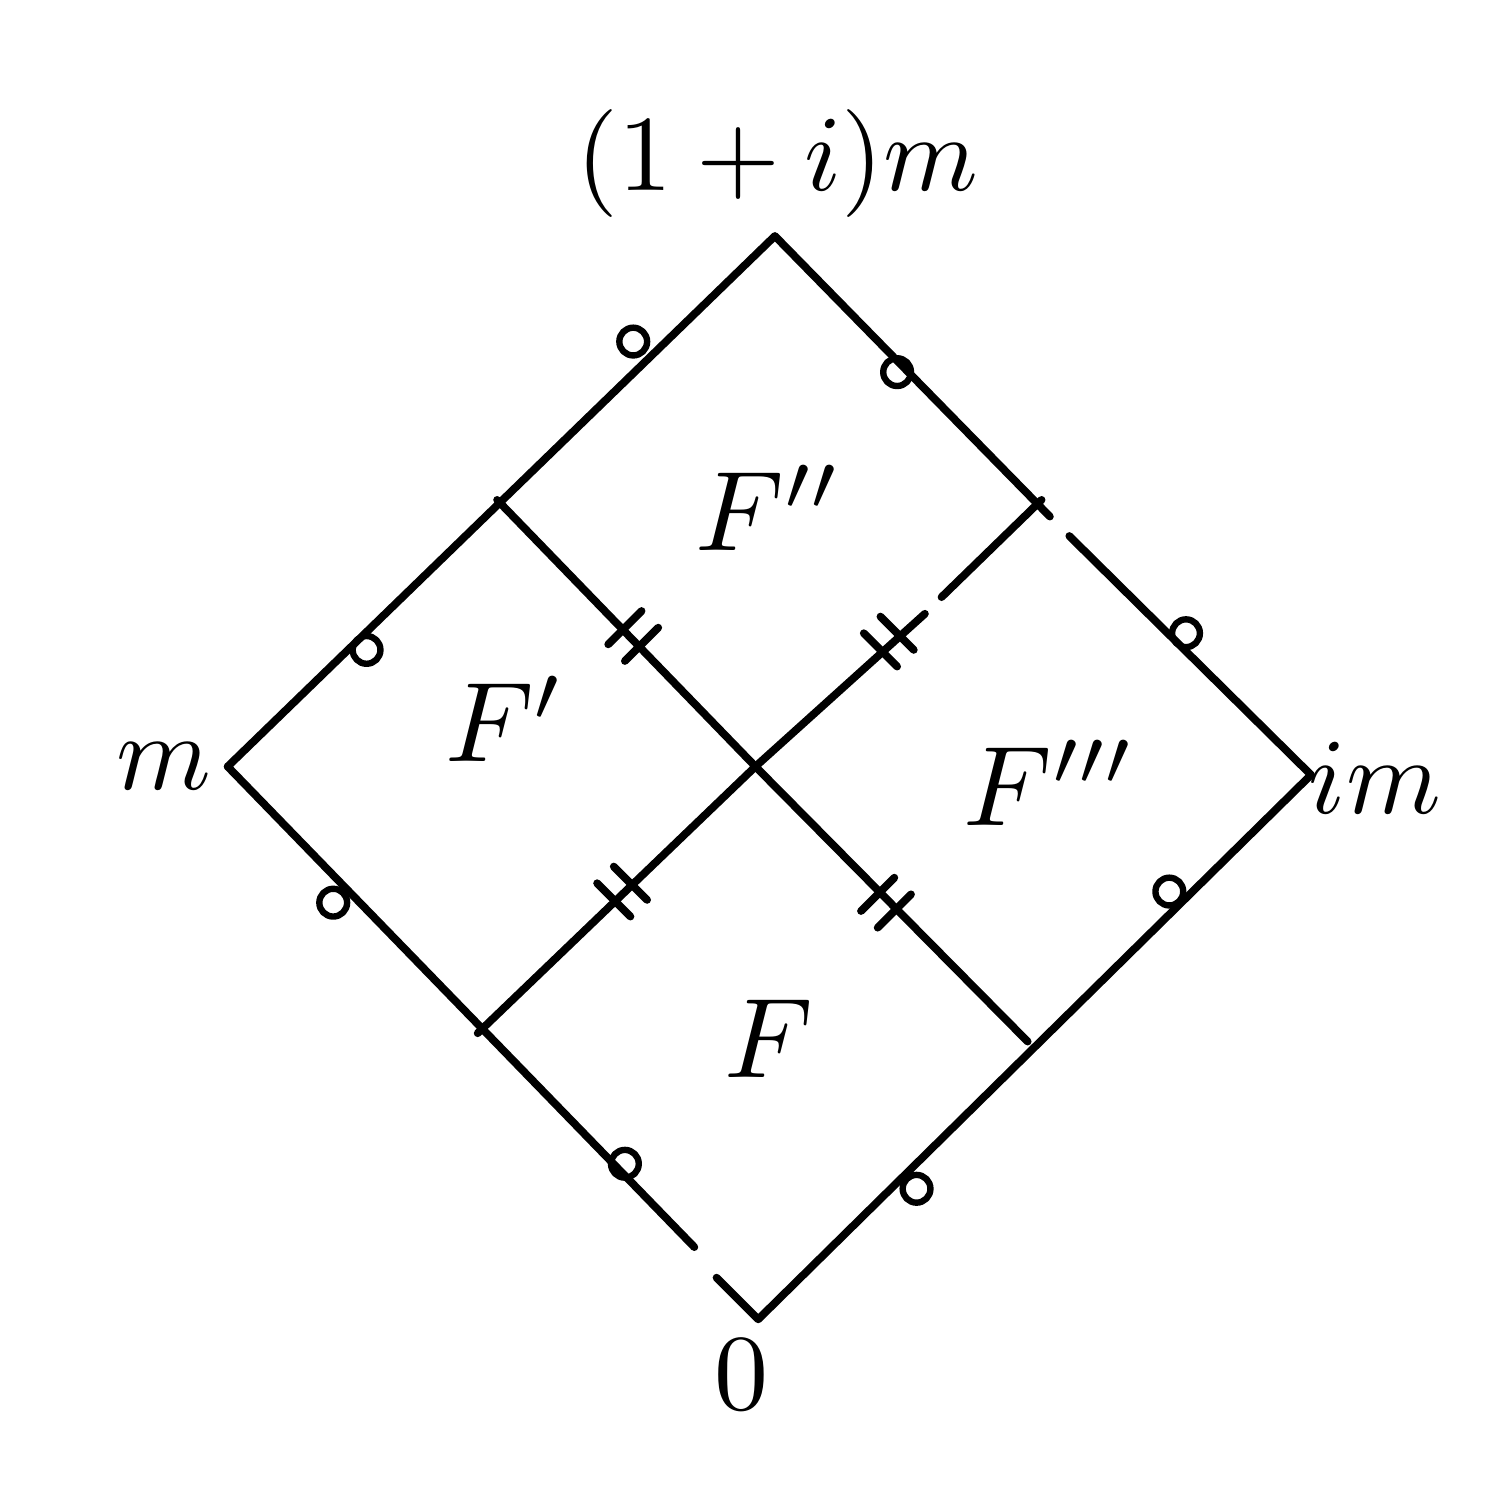
\begin{tikzpicture}[x=1bp,y=-1bp,line cap=round,line join=round]
\path[use as bounding box] (0,0) rectangle (520,520);
\begin{pgfinterruptboundingbox}
\draw[line width=2.8bp] (72,266) -- (269,75) -- (368,176);
\draw[line width=2.8bp] (375,183) -- (462,269) -- (263,465) -- (248,450);
\draw[line width=2.8bp] (240,439) -- (72,266);
\draw[line width=2.8bp] (169,170) -- (262,266) -- (360,365);
\draw[line width=2.8bp] (365,170) -- (329,205);
\draw[line width=2.8bp] (323,211) -- (262,266) -- (162,362);
\draw[line width=2.3bp] (218,113) circle[radius=5bp];
\draw[line width=2.3bp] (313,124) circle[radius=5bp];
\draw[line width=2.3bp] (122,224) circle[radius=5bp];
\draw[line width=2.3bp] (417,218) circle[radius=5bp];
\draw[line width=2.3bp] (110,315) circle[radius=5bp];
\draw[line width=2.3bp] (411,311) circle[radius=5bp];
\draw[line width=2.3bp] (215,409) circle[radius=5bp];
\draw[line width=2.3bp] (320,418) circle[radius=5bp];
\draw[line width=2.8bp] (209,222) -- (221,210);
\draw[line width=2.8bp] (215,228) -- (227,216);
\draw[line width=2.8bp] (301,218) -- (313,230);
\draw[line width=2.8bp] (307,212) -- (319,224);
\draw[line width=2.8bp] (205,308) -- (217,320);
\draw[line width=2.8bp] (211,302) -- (223,314);
\draw[line width=2.8bp] (300,318) -- (312,306);
\draw[line width=2.8bp] (306,324) -- (318,312);
\node[inner sep=0pt,outer sep=0pt,anchor=center] at (267,173) {\scalebox{4.1}{\ensuremath{F''}}};
\node[inner sep=0pt,outer sep=0pt,anchor=center] at (172,249) {\scalebox{4.1}{\ensuremath{F'}}};
\node[inner sep=0pt,outer sep=0pt,anchor=center] at (368,272) {\scalebox{4.1}{\ensuremath{F'''}}};
\node[inner sep=0pt,outer sep=0pt,anchor=center] at (267,364) {\scalebox{4.1}{\ensuremath{F}}};
\node[inner sep=0pt,outer sep=0pt,anchor=center] at (49,266) {\scalebox{3.9}{\ensuremath{m}}};
\node[inner sep=0pt,outer sep=0pt,anchor=center] at (270,49) {\scalebox{3.9}{\ensuremath{(1+i)m}}};
\node[inner sep=0pt,outer sep=0pt,anchor=center] at (485,270) {\scalebox{3.9}{\ensuremath{im}}};
\node[inner sep=0pt,outer sep=0pt,anchor=center] at (257,485) {\scalebox{3.9}{\ensuremath{0}}};
\end{pgfinterruptboundingbox}
\end{tikzpicture}
}\end{center}
In particular cases, however, another distribution may be more advantageous.

\Article{16}
If $f,f',f''$, etc., are all the primitive residues of the modulus $m$, then
\SourceLeaf{328}
\[
\begin{aligned}
&S(z+\tfrac fm,\ z'+\tfrac fm,\ z''+\tfrac fm,\ \text{etc.})\\
&+S(z+\tfrac{f'}m,\ z'+\tfrac{f'}m,\ z''+\tfrac{f'}m,\ \text{etc.})\\
&+S(z+\tfrac{f''}m,\ z'+\tfrac{f''}m,\ z''+\tfrac{f''}m,\ \text{etc.})\\
&+\text{etc.}\\
&=S(mz,mz',mz'',\ \text{etc.}
\end{aligned}
\]
